\documentclass{standalone}

\usepackage{tikz}
\usepackage{scalefnt}

\usetikzlibrary{scopes}

\begin{document}

{\scalefont{0.5}
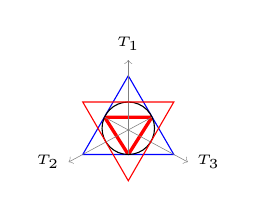
\begin{tikzpicture}[
  sides/.style={draw=blue, font=\small},
  band/.style={draw=red, font=\footnotesize},
  thickband/.style={draw=red, font=\footnotesize, very thick},
  axis/.style={very thin, draw=gray,font=\tiny},
  ]
    %% Free body diagram of M

      % {[axis,->]
      %   \draw (0,0) -- (-1/1.73,-1/3) node[right] {$T_{2}$};
      %   \draw (M) -- ++(2,0) node[right] {$+x$};
      % }

  % Triangle
  \draw[sides]
     (-1/1.73,-1/3) -- (1/1.73,-1/3) -- (0,2/3) node (top) {} -- cycle;

  

  \begin{scope}
   \clip (0,0) circle (1/3);
   \draw[thickband] (0.3, 0.14) -- (-0.3, 0.14) -- (0, -1/3) -- cycle;
  \end{scope}

  % Inscribed circle
  \draw (0,0) circle (1/3);

  % Energy axis
  {[axis,->]
    \draw (0, -1/3) -- ++ (90:1.2) node[above] {$T_{1}$};
    \draw (0.3, 0.14) -- ++ (-151.7:1.2) node[left] {$T_{2}$};
    \draw (-0.3, 0.14) -- ++ (-28.3:1.2) node[right] {$T_{3}$};
  }

  \begin{scope}[rotate=180]
    \draw[band]
    (-1/1.73,-1/3) -- (1/1.73,-1/3) -- (0,2/3) -- cycle;
  \end{scope}


\end{tikzpicture}
}
\end{document}